\documentclass {article}

\usepackage{framed}
\usepackage{amsmath}
\usepackage{amssymb}
\usepackage{graphicx}
\usepackage{float}

\title{Assignment 3 for CS224d}
\author{Lifu Huang}
\date{April 2016}

\begin{document}
\maketitle
\section{RNN's(Recursive Neural Network)}
\subsection*{(a)}
\begin{align*}
\delta^{(s)} &= \hat{y} - y \\
\delta^{(1)} &= f'(h^{(1)}) \circ (U^T \delta^{(s)} + \delta_{above}) \\
\delta_{below} &= (W^{(1)})^T \delta^{(1)}
\\
\nabla_U J &= \delta^{(s)} (h^{(1)})^T \\
\nabla_{b^{(s)}} J &= \delta^{(s)} \\
\nabla_{W^{(1)}} J &= \delta^{(1)} \left[(h^{(1)}_{left})^T\  (h^{(1)}_{right})^T\right] \\
\nabla_{b^{(1)}} J &= \delta^{(1)} \\
\nabla_{\left[L_{left}^T\ L_{right}^T\right]^T} J &= \delta_{below} \\
\end{align*}
\subsection*{(b)}
Please see code files for details.
\newpage
\subsection*{(c)}
\subsubsection*{(a)}
\begin{figure}[H]
\centering
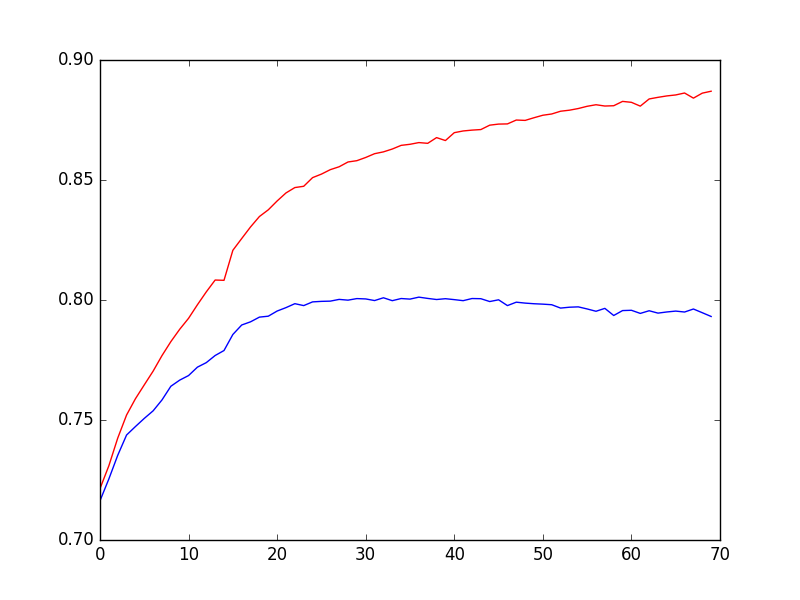
\includegraphics[width=0.7\linewidth]{ps3_1_c_a}
\caption{Accuracy on Training and Dev Set over Epochs}
\label{fig:ps3_1_c_a}
\end{figure}
\subsubsection*{(b)}
Beacause training for too many epochs may lead to the problem of over fitting.
\subsubsection*{(c)}
\begin{figure}[H]
\centering
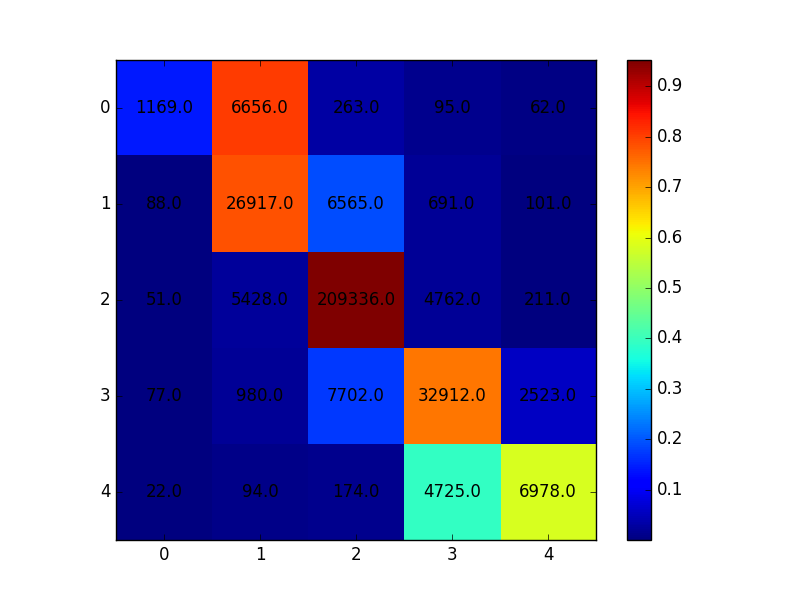
\includegraphics[width=0.7\linewidth]{ps3_1_c_c_train}
\caption{Confusion Matrix on Training Set}
\label{fig:ps3_1_c_c_train}
\end{figure}
\begin{figure}[H]
\centering
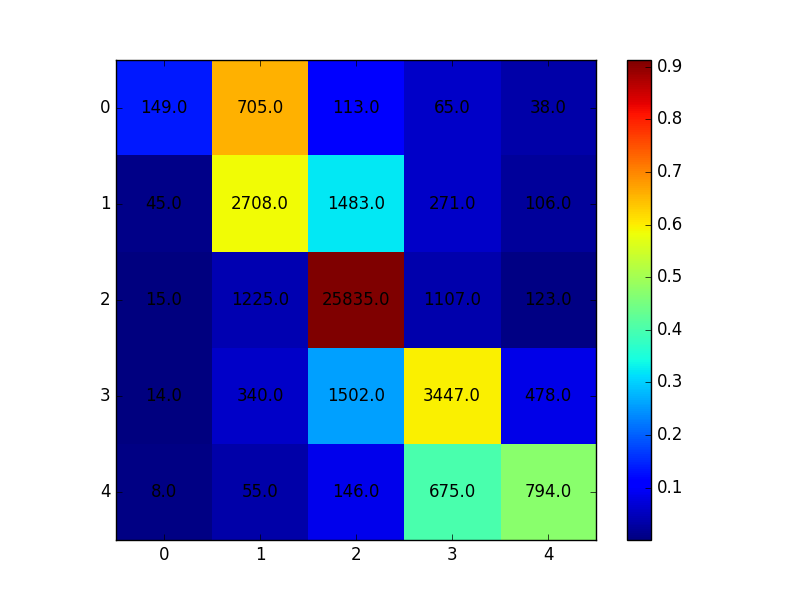
\includegraphics[width=0.7\linewidth]{ps3_1_c_c_dev}
\caption{Confusion Matrix on Dev Set}
\label{fig:ps3_1_c_c_dev}
\end{figure}
\subsubsection*{(d)}
\begin{figure}[H]
\centering
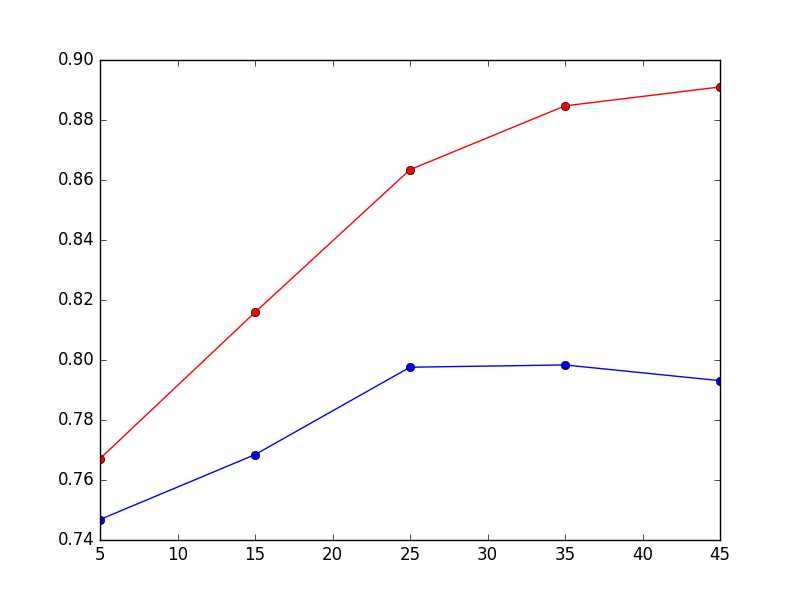
\includegraphics[width=0.7\linewidth]{ps3_1_c_d}
\caption{Accuracy on Training and Dev Set over wvecDims}
\label{fig:ps3_1_c_d}
\end{figure}
\newpage

\section{2-Layer Deep RNN's}
\subsection*{(a)}
\subsection*{(b)}
\subsection*{(c)}
\subsection*{(d)}
\subsection*{(e)}
\subsection*{(f)}

\section{Extra Credit: Recursive Neural Tensor Networks}
\end{document}